% Created 2016-09-18 Sun 20:04
\documentclass[11pt]{article}
\usepackage[utf8]{inputenc}
\usepackage[T1]{fontenc}
\usepackage{fixltx2e}
\usepackage{graphicx}
\usepackage{longtable}
\usepackage{float}
\usepackage{wrapfig}
\usepackage{rotating}
\usepackage[normalem]{ulem}
\usepackage{amsmath}
\usepackage{textcomp}
\usepackage{marvosym}
\usepackage{wasysym}
\usepackage{amssymb}
\usepackage{hyperref}
\tolerance=1000
\usepackage{siunitx}
\author{Willy Bernal Heredia - National Renewable Energy Laboratory}
%\author{Author A}
\date{\today}
\title{MLE+: Tutorial}
\hypersetup{
  pdfkeywords={},
  pdfsubject={},
  pdfcreator={Emacs 25.1.1 (Org mode 8.2.10)}}
\begin{document}

\maketitle
\tableofcontents



\section{Introduction}
\label{sec-1}

MLE+ is an open-source Matlab/Simulink toolbox for building energy simulation, analysis, optimization and control design. At the core of MLE+ are co-simulation interfaces with multiple building energy simulation programs such as \href{http://apps1.eere.energy.gov/buildings/energyplus/}{EnergyPlus}. MLE+ provides a Simulink library with a S-Function block for easy drag-and-drop implementation. Figure \ref{fig:overview} illustrates the overall structure of MLE+.

\textbf{Note:} This version of MLE+ does not provide a graphical interface. 

\begin{figure}[htb]
\centering
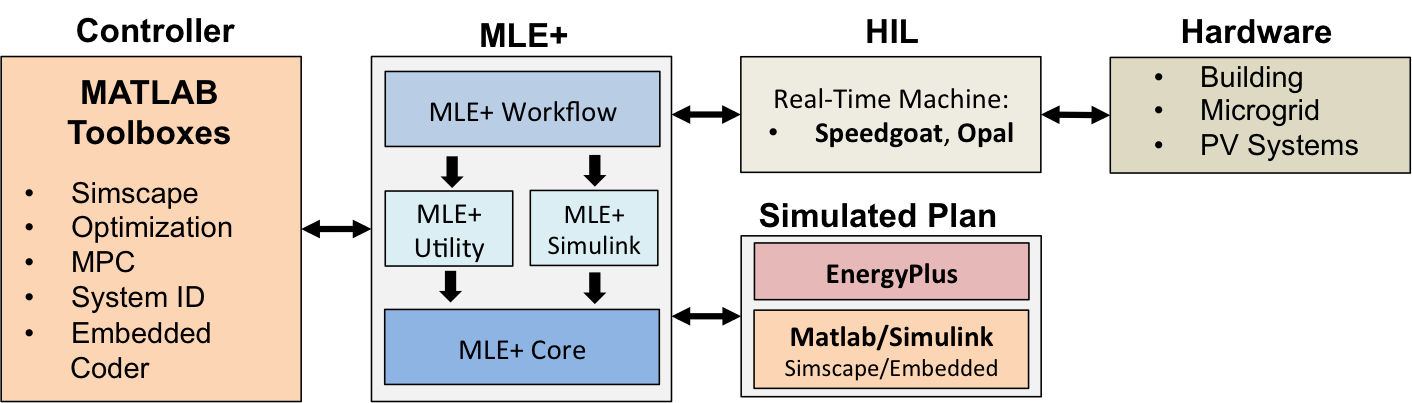
\includegraphics[width=.9\linewidth]{./figs/overview.pdf}
\caption{\label{fig:overview}MLE+ interfaces control system toolboxes with building models and systems.}
\end{figure}

MLE+ is designed for engineers and researchers who are familiar with
Matlab and Simulink and want to use these software tools in building
energy research.  MLE+ is particularly useful for:
\begin{enumerate}
\item \textbf{Simulation configuration:} The MLE+ front-end streamlines the
configuration process of linking the building model and the
controllers by abstracting the necessary parameters from the
co-simulation. This reduces setup time and configuration
problems.
\item \textbf{Controller design:} MLE+ provides a control development workflow as
well as graphical front-ends for designing advanced control
strategies for buildings, in which the building simulation is
carried out by dedicated simulation software, such as EnergyPlus,
while the controllers are implemented in Matlab or Simulink.
\item \textbf{Simulation-based optimization:} MLE+ can be used to find optimal
parameters or control sequences for building system designs,
using simulation-based nonlinear optimization.
\item \textbf{Data analysis:} Simulation output data from EnergyPlus can be
aggregated, analyzed and visualized in Matlab.
\item \textbf{Building Energy Management System Interface:} MLE+ provides a
BACnet interface to develop and implement control methods for
real building equipment.
\item \textbf{Matlab/Simulink environment:} MLE+ allows complete access to the
Matlab environment and toolboxes such as Global Optimization
Toolbox, System Identification Toolbox and Model Predictive
Control Toolbox. The user can step through the code for debugging
and pause the co-simulation at any time.
\end{enumerate}


\section{System Requirements}
\label{sec-2}

\begin{itemize}
\item Windows Operating System. Currently, MLE+ is only supported in
Windows. However, we are working in making MLE+ compatible in the
Linux and Mac OS platforms.
\item MLE+ requires Matlab and/or Simulink of recent versions.  MLE+ uses
the \href{http://www.mathworks.com/matlabcentral/fileexchange/27758}{GUI Layout Toolbox}.  This is included in the MLE+
distribution.  MLE+ has been tested in Matlab 2011a and 2012a
versions\footnote{The GUI Layout Toolbox requires 2010a or
  future version of Matlab. If you find any problems, please contact
  the authors for further assistance}.
\item Java must be enabled in Matlab. By default, Java is already enabled
in Matlab, so no further action is required.  The Java socket
library is used by MLE+ for communication with EnergyPlus.
\item EnergyPlus version 7.1.0 (latest). MLE+ should work well with
previous versions of EnergyPlus: versions 7.0.0 and 6.0.0.  However,
it has not been tested thoroughly.  We strongly recommend to
download EnergyPlus 7.1.0 as the example files correspond to this
version.
\end{itemize}


\section{Installation}
\label{sec-3}

\begin{enumerate}
\item Download the latest version from
\url{https://github.com/mlab/mlep_v1.1/zipball/master}
or clone the repository \url{https://github.com/mlab/mlep_v1.1}
\item Extract all files to a directory in your computer.  Call this folder
\texttt{/mlep}.
\item Open Matlab and change the current directory to the \texttt{/mlep/MLE+} folder
that has just been created.  In Matlab, run the installation script
\texttt{installMep.m} and follow the instructions.
\end{enumerate}

\subsection{WINDOWS}
\label{sec-3-1}

\begin{enumerate}
\item This will install the
GUI Layout Toolbox and add the necessary paths to the Matlab
environment automatically. After that, the installation screen in 
Figure \ref{fig:installScreen} will appear. Here you need to specify the 
paths to EnergyPlus main Directory and the path to the folder with 
Java binaries. Also, this will replace
your \texttt{RunEPlus.batch} file (in Windows).
\end{enumerate}

\begin{figure}[htb]
\centering
\includegraphics[width=.9\linewidth]{figs/installation.png}
\caption{\label{fig:installScreen}Windows MLE+ Installation Screen.}
\end{figure}

\subsection{MAC}
\label{sec-3-2}

\begin{enumerate}
\item This will install the
GUI Layout Toolbox and add the necessary paths to the Matlab
environment automatically. After that, the installation screen in 
Figure \ref{fig:installScreenMAC} will appear. Here you need to specify the 
paths to EnergyPlus main Directory.
\item In MAC distributions, the orginal \texttt{runenergyplus} file in your
EnergyPlus Distribution (e.g. \texttt{\textbackslash{}Applications\textbackslash{}EnergyPlus\textbackslash{}runenergyplus}) makes sure 
the EnergyPlus result files are written to the \texttt{\textbackslash{}Output} folder and \texttt{.mat} files
are not deleted.
\end{enumerate}

\begin{figure}[htb]
\centering
\includegraphics[width=.9\linewidth]{figs/installationMAC.pdf}
\caption{\label{fig:installScreenMAC}MAC OS MLE+ Installation Screen.}
\end{figure}

\subsection{MAnual Installation}
\label{sec-3-3}

\begin{enumerate}
\item Depending on your Matlab distribution, you might not be able to use the GUILayout
\end{enumerate}
tool required to open the MLE+ front-end. If you run into some problems installing try 
using the manual installation. You would need to follow this instructions .


\section{Tutorial: Shading Control Example}
\label{sec-4}

In the following tutorial example, we will walk you through the steps
to set up a co-simulation session with EnergyPlus from Matlab.  We
will then design a controller in MLE+ for actuating the window blinds of a
building simulated in EnergyPlus.

\subsection{The Building}
\label{sec-4-1}

A single-storied building shown in Figure \ref{fig:buildingcad}
consists of three zones with a total floor area of 130 \{m$^{\text{2}}$\} 
\#\SI{130}{\meter\squared}.
The West zone of the building consists of a
large window equipped with blinds/shades and is subject to strong
solar radiation during the day.  The goal is to control the window
shade deployment of the West zone such that the transmitted solar
radiation (through the window) never exceeds a certain threshold.  The
window blinds can be controlled using two EnergyPlus variables:
\begin{itemize}
\item \texttt{Shading\_Deployment\_Status} controls whether the blinds are deployed
or not;
\item \texttt{ShadeAngle\_Schedule} controls the slat angle so it is perpendicular
to the incident solar radiation whenever the blinds are deployed.
\end{itemize}


\begin{figure}[htb]
\centering
\includegraphics[width=.9\linewidth]{figs/buildingcad.jpg}
\caption{\label{fig:buildingcad}EnergyPlus window shading control model.}
\end{figure}

We will design a controller in MLE+ which monitors the angle and
intensity of the solar radiation incident on the West zone window.  If
the incident solar radiation exceeds a certain threshold, the blinds
will be deployed and the shade angle will be set to reduce the
possibility of glare.


\subsection{The MLE+ Control Design Workflow}
\label{sec-4-2}

The control design workflow of MLE+ defines a sequence of steps for
designing a controller in Matlab for a building model simulated by
EnergyPlus.  A graphical front-end is provided to support this
workflow.  To start the front-end, execute the command \texttt{mlep} in
Matlab. This will open a graphical interface as shown in Figure
\ref{fig:startupgui}.


\begin{figure}[htb]
\centering
\includegraphics[width=.9\linewidth]{figs/start.png}
\caption{\label{fig:startupgui}Graphical front-end for the MLE+ control design workflow.}
\end{figure}



\subsection{Set Up EnergyPlus Simulation Model}
\label{sec-4-3}

First, we need to specify the EnergyPlus building model and the
weather profile to be used for simulation (Figure \ref{fig:startupgui}).
\begin{itemize}
\item Click the button \textbf{Select IDF file} and select the file
\texttt{EMSWindowShadeControl.idf} located in the folder \texttt{/ShadingProject}.
\item Click the button \textbf{Select weather file} and select the weather file
\texttt{USA\_IL\_Chicago-OHare.Intl.AP.725300\_TMY3.epw}.  We will use the
weather profile of Chicago for our simulation.
\end{itemize}


\subsection{Configure Input and Output Variables Between EnergyPlus and Matlab}
\label{sec-4-4}

We will set up the input and output variables to be exchanged between
EnergyPlus and Matlab for co-simulation. An input variable serves as
an input to EnergyPlus at each step of the co-simulation, while output
variables are those which can be repeatedly read from EnergyPlus to
monitor its internal state.

\begin{figure}[htb]
\centering
\includegraphics[width=.9\linewidth]{figs/control.png}
\caption{\label{fig:control}MLE+ control design tab.}
\end{figure}

\begin{enumerate}
\item Select the Control Tab (Figure \ref{fig:control})
\item In the Control Tab, push the \textbf{Variable} button to open the Variable
Configuration Window (Figure \ref{fig:variable}).
\item Load the \texttt{.idf} file by pushing the \textbf{Load IDF} button. This
will list the available \texttt{ExternalInterface:Schedule},
\texttt{ExternalInterface:Actuator} and \texttt{ExternalInterface:Variable}
objects from the idf file. It will also list the available
\texttt{Output:Variable} objects.
\item Add the necessary inputs and outputs to have the settings specified
in (Figure \ref{fig:input}) and (Figure \ref{fig:output}),
respectively.  In this example, we specify
\texttt{Shading\_Deployment\_Status} and \texttt{ShadeAngle\_Schedule} as the inputs
to EnergyPlus as these are the variables that we will control
through MLE+. Make sure your configuration is exactly the same as
the one shown in (Figure \ref{fig:input}) and (Figure
\ref{fig:output}).
\item Once the input and output variables had been set, push the green
button \textbf{Write Variables.cfg}. This file will create a file
with the communication configuration between Matlab and
EnergyPlus. It should be printed in the Matlab command line.
\item Close the Variable Configuration Window. Either click on the \textbf{Close Screen}
   or the \textbf{X}.
\end{enumerate}


In MLE+, an alias can be specified for each of the variables (Figure \ref{fig:input} and Figure \ref{fig:output}). 
The alias allows the user to reference a variable with a more intuitive name and avoid the intricate names specified by EnergyPlus.
For instance, the EnergyPlus variable \texttt{Zn001\_Wall001\_Win001\_Shading\_Deployment\_Status} can be assigned a more intuitive name as \texttt{ShadeStatus}.

\begin{figure}[htb]
\centering
\includegraphics[width=.9\linewidth]{figs/variables.png}
\caption{\label{fig:variable}Variable configuration window.}
\end{figure}


\begin{figure}[htb]
\centering
\includegraphics[width=.9\linewidth]{figs/variableInput.png}
\caption{\label{fig:input}Configuration of input variables to EnergyPlus.}
\end{figure}


\begin{figure}[htb]
\centering
\includegraphics[width=.9\linewidth]{figs/variableOutput.png}
\caption{\label{fig:output}Configuration of output variables to EnergyPlus.}
\end{figure}



\subsection{Design a Shading Controller}
\label{sec-4-5}

In the control tab, we will specify
the building controller, implemented in Matlab, for our building model (Figure \ref{fig:control1}).
\begin{enumerate}
\item Push the button \textbf{Load Control File} and select the file
\texttt{control\_file\_blind\_angle.m}.  This file contains the Matlab code
for the shading controller.
\item View and edit this file by clicking the button \textbf{Edit Control File.}
You can also create a template file for your own feedback loop by clicking 
on \textbf{Create Control File.} This creates the file \texttt{controlFile.m}.
\end{enumerate}


The input and output variables specified by the user are referred to
by their aliases throughout the control file as shown in Figure
\ref{fig:code}.  In the code snippet shown in Figure \ref{fig:code}
the value of the incident solar radiation is compared against the
threshold (\SI{100}{\watt\per\meter\squared}) to determine if the
shades will be deployed.


\begin{figure}[htb]
\centering
\includegraphics[width=.9\linewidth]{figs/control1.png}
\caption{\label{fig:control1}MLE+ control design tab.}
\end{figure}


\begin{figure}[htb]
\centering
\includegraphics[width=.9\linewidth]{figs/code.pdf}
\caption{\label{fig:code}Matlab code snippet of the shading controller (notice alias variables).}
\end{figure}



\subsection{Simulation and Assessment}
\label{sec-4-6}

\begin{figure}[htb]
\centering
\includegraphics[width=.9\linewidth]{figs/simulate.png}
\caption{\label{fig:simulate}Plot and analyze simulation results of EnergyPlus.}
\end{figure}



Once a control design has been completed, we can run the simulation or
step through it using the Matlab debugging environment.

\begin{enumerate}
\item Click on the tab \textbf{Simulate} then click on button \textbf{Run Simulation}
This will call EnergyPlus to run the building energy simulation
with the parameters we have specified.
\item A Windows command window will open and will show the progress of
the simulation.
\item After the co-simulation has finished, MLE+ extracts and parses all
output variables generated by EnergyPlus, then lists them in a
listbox (see Figure \ref{fig:simulate}).  Select one or multiple
variables, then click the button \textbf{Plot} to display them on the screen.
\item You can also save the data to the Matlab workspace by clicking the
buttons \textbf{Save all} or \textbf{Save Selected}
\item The building geometry is visualized in tab \textbf{Building.}
\end{enumerate}


Note that MLE+ decouples the simulation engine and the controller
implementation.  This way we can tune the control scheme in Matlab,
then assess its performance by running multiple simulations without
the need of modifying the EnergyPlus file.



\subsection{Load, Save and Reset Project Data}
\label{sec-4-7}

At the bottom of the window, you can find buttons to load a control
design project from a file, save a project to a file, and reset the
current project data.  A project file has the extension \texttt{.prj} and
contains all essential information of a control design project.

\begin{enumerate}
\item \textbf{Load Project:} open previously saved projects.
\item \textbf{Save Project:} save all the configuration settings which have been
entered so far to a file.  Note that this does not save your
controller file, or your \texttt{.idf} file.
\item \textbf{Reset Project:} empty all fields in the graphical front-end.  Note that this will
not erase the current project file, but only reset the
configuration settings in the graphical front-end.
\item \textbf{Exit:} exit the program.
\end{enumerate}


For your convenience, a project file for the tutorial example is
included in the distribution.  You can load the project file
\texttt{ShadingProject.prj} and switch directly to the tab \textbf{Simulate} to
run a simulation of the control design.




\section{Other Examples}
\label{sec-5}

\subsection{Legacy Example}
\label{sec-5-1}
This folder contains the original example distributed with MLE+ Legacy. This example does
not make use of the MLE+ front end. You can run this example by
executing runsimple.m in Matlab. This example sets the Temperature Setpoints for a small building. 


\subsection{Green Scheduling vs. Uncoordinated Control}
\label{sec-5-2}
Here we compared two different binary (ON/OFF) controls for keeping
the temperature of a small building inside the comfort level. 
Green Scheduling is a control
scheme designed to reduce peak power consumption while satisfying the
temperature conditions. You can load these projects by using the \textbf{Load
Project} button.


\subsection{MPC vs. Proportional Control}
\label{sec-5-3}
These two cases implement continuous control schemes. The first control is a Model 
Predictive controller using built-in functions in
Matlab. This is compared against a very simple proportional feedback
loop. The model for the first strategy was generated using the \textbf{System
Identification tab} in MLE+. This tab allows you to design the disturbances
you feed your model for SYSID. Then, you can import this model directly into the Matlab's built-in
system identification toolbox.  
% Emacs 25.1.1 (Org mode 8.2.10)
\end{document}
